\hypertarget{appendix-cb5af353ef77}{}
\section*{10 - Probability and Monte Carlo - Visual Recall}
\section{Probability and uncertainty --- visual recall}\label{appendix-cb5af353ef77-probability-and-uncertainty-visual-recall}

\pandocbounded{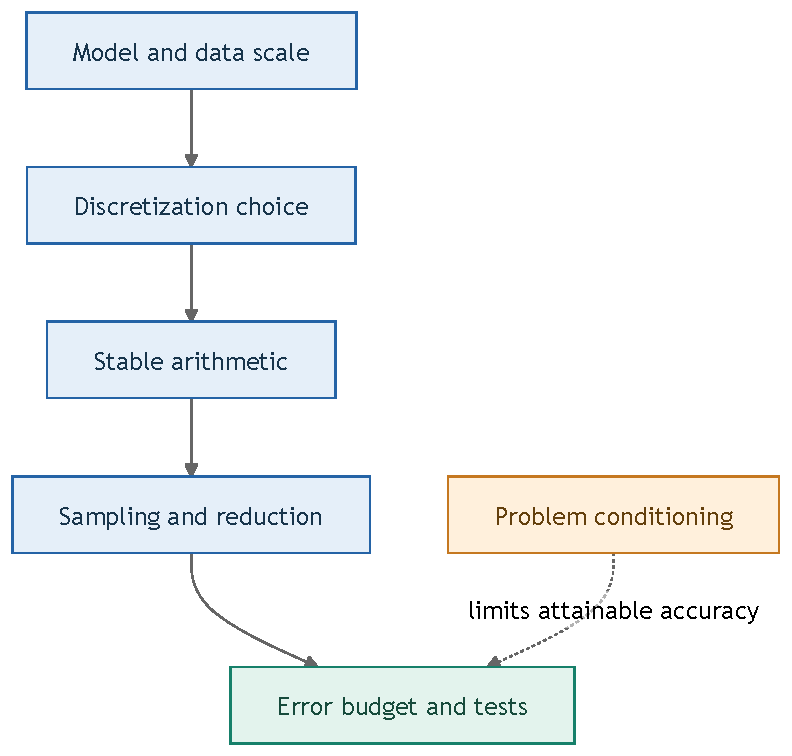
\includegraphics[keepaspectratio,alt={Diagram}]{../Assets/Print/d9b64ab5b2cf6dd86db7e3fae4db06821352cc5eea4460cd629a8db38d181c15.pdf}}

Shortest route: start with a model of outcomes, then ask what distribution the computer actually sampled, how it weighted each sample, and what evidence supports the estimate.

\subsection{Reconstruct the chain}\label{appendix-cb5af353ef77-reconstruct-the-chain}

\texttt{(Ω,\ F,\ P)} describes outcomes, measurable events, and their probabilities. A random variable maps outcomes into numbers; a random vector preserves their joint behavior. A PMF assigns point mass to discrete values; a PDF gives density relative to a stated measure; a CDF accumulates probability and exists even when no PDF does.

Conditioning changes the information available. Independence means joint probability factors, not merely that events are disjoint. Bayes reverses the conditioning direction by multiplying likelihood by prior and normalizing over alternatives.

Expectation is a probability-weighted center. Variance is mean squared spread. Covariance records coupled variation; correlation divides it by both standard deviations but only captures linear association. For a vector, covariance is symmetric PSD because \texttt{aᵀΣa\ =\ Var(aᵀX)\ ≥\ 0}.

Bernoulli describes one binary outcome; binomial counts IID Bernoulli successes. Uniform has constant density in its declared measure. Gaussian describes a quadratic-distance bell shape. Exponential waiting times are memoryless; Poisson counts belong to the corresponding constant-rate process. A multivariate Gaussian's covariance sets ellipse/ellipsoid orientation and scale.

The computational chain is:

\begin{verbatim}
seed/state or keyed input → finite random bits → sample transform → actual PDF and measure
                              → weighted contribution f(X)/p(X) → average → uncertainty/error report
\end{verbatim}

Every arrow carries assumptions. A wrong PDF or measure can bias the result. A low-variance estimator can still be biased. Correlated observations change the standard error. Confidence intervals do not repair a wrong expectation.

\subsection{Formula prompts}\label{appendix-cb5af353ef77-formula-prompts}

{\def\LTcaptype{none} % do not increment counter
\begin{longtable}[]{@{}
  >{\raggedright\arraybackslash}p{(\linewidth - 2\tabcolsep) * \real{0.5000}}
  >{\raggedright\arraybackslash}p{(\linewidth - 2\tabcolsep) * \real{0.5000}}@{}}
\toprule\noalign{}
\begin{minipage}[b]{\linewidth}\raggedright
Prompt
\end{minipage} & \begin{minipage}[b]{\linewidth}\raggedright
Reconstruct
\end{minipage} \\
\midrule\noalign{}
\endhead
\bottomrule\noalign{}
\endlastfoot
Conditioning & \texttt{P(A\textbar{}B)=P(A∩B)/P(B)}; chain rule multiplies successive conditional probabilities. \\
Bayes & \texttt{P(H\textbar{}E)=P(E\textbar{}H)P(H)/ΣᵢP(E\textbar{}Hᵢ)P(Hᵢ)}. \\
Expected transform & \texttt{E{[}g(X){]}\ =\ Σg(x)p(x)} or \texttt{∫g(x)p(x)dx}. \\
Variance/covariance & \texttt{Var(X)=E{[}X²{]}−E{[}X{]}²}; \texttt{Cov(X,Y)=E{[}XY{]}−E{[}X{]}E{[}Y{]}}. \\
Linear propagation & \texttt{E{[}AX+b{]}=Aμ+b}; \texttt{Cov(AX+b)=AΣAᵀ}; local nonlinear approximation uses \texttt{JΣJᵀ}. \\
Importance estimate & \texttt{I=∫f\ dx=Eₚ{[}f(X)/p(X){]}}; average contributions and divide by the actual sampling density. \\
Monte Carlo error & IID finite-variance mean has \texttt{Var(Ȳ)=σ²/N}, \texttt{SE=σ/√N}; four times samples halves SE. \\
Estimator quality & \texttt{MSE\ =\ variance\ +\ bias²}. \\
Bessel/Welford & Unbiased sample variance uses \texttt{M₂/(n−1)}; update with \texttt{δ=x−μ}, \texttt{μ←μ+δ/n}, \texttt{M₂←M₂+δ(x−μ)}. \\
Error metrics & MSE squares; RMSE returns original units; MAE uses absolute error; relative metrics fail or need policy near zero. \\
\end{longtable}
}

\subsection{Fast error checks}\label{appendix-cb5af353ef77-fast-error-checks}

\begin{itemize}
\tightlist
\item
  Does a density integrate to one in the stated coordinate measure? Is its unit inverse measure?
\item
  Are the samples distributed according to the PDF used in the weight?
\item
  Is a stated confidence interval fixed-sample, and are IID/normal or approximation assumptions plausible?
\item
  Is covariance symmetric PSD? Does singular mean invalid, or valid but lower-rank?
\item
  Are sample and population variance being confused? Is a single run being mistaken for evidence of variance reduction?
\item
  Is a ``Gaussian'' a normalized probability model or merely a rendering kernel?
\end{itemize}

\subsection{Targeted backlinks}\label{appendix-cb5af353ef77-targeted-backlinks}

\begin{itemize}
\tightlist
\item
  \href{Continuous\%20Notes/Computing\%20Foundations\%20-\%20From\%20Bits\%20to\%20C++\%20and\%20Systems\%20APIs\#A\%20direction\%20can\%20exist\%20even\%20when\%20the\%20naive\%20length\%20overflows}{stable numerics}
\item
  \hyperref[01-foundations-i-ch018-an-inverse-can-exist-and-still-amplify-uncertainty]{conditioning}
\item
  \hyperref[01-foundations-i-ch019-coordinates-can-change-while-the-geometric-object-stays-still]{coordinate changes}
\item
  \hyperref[01-foundations-i-ch020-positive-definiteness-is-a-structural-promise]{positive definiteness}
\item
  \hyperref[01-foundations-i-ch020-diagonalization-leads-to-the-stronger-symmetric-spectral-theorem]{covariance eigenstructure}
\end{itemize}

Parts covered by supplied sources: 901--1000. The numerical continuation and figure index below complete this received phase.

\subsection{Source-provided recall and compact formula reference}\label{appendix-cb5af353ef77-source-provided-recall-and-compact-formula-reference}

\subsection{Supplied concise recall summary}\label{appendix-cb5af353ef77-supplied-concise-recall-summary}

The mathematical core is the probability space \((\Omega,\mathcal F,P)\), random variables defined on that space, and probability laws for their values.

Conditional probability changes the reference information. Independence is a factorization property. PMFs assign masses to discrete values, while PDFs assign density relative to a measure. CDFs accumulate probability and exist for every real-valued random variable.

Expected value describes the weighted centre. Variance describes squared spread. Covariance describes coupled spread. Correlation standardizes covariance but does not measure every form of dependence.

Bernoulli models one binary trial. Binomial models the count of successes in independent identically distributed Bernoulli trials. Uniform models constant density over a region. Gaussian models a particular smooth bell-shaped distribution. Exponential models memoryless waiting times. Poisson models event counts under its defining assumptions.

A multivariate Gaussian combines mean, covariance, and correlations into a joint distribution. Positive-definite covariance permits a full-dimensional nonsingular Gaussian density. Singular PSD covariance describes a distribution confined to a lower-dimensional affine subspace.

Key engineering invariants: all probabilities are valid and normalized; PDF units match the integration measure; covariance is symmetric PSD; Gaussian density evaluation avoids unnecessary inversion; nonfinite inputs and singular cases are explicit; sampling tests use statistical tolerances rather than exact equality.

\subsection{Supplied compact formula reference}\label{appendix-cb5af353ef77-supplied-compact-formula-reference}

Random generation and transformations

\[
 U\sim\mathcal U(0,1),\qquad X=F^{-1}(U) 
\]

\[
 p_Y(g(x)) = \frac{p_X(x)}{|\det J_g(x)|} 
\]

Importance sampling

\[
 \widehat I_N= \frac1N\sum_i\frac{f(X_i)}{p(X_i)} 
\]

\[
 \operatorname{Var}(\widehat I_N) = \frac1N \left[ \int\frac{f(x)^2}{p(x)}dx-I^2 \right] 
\]

Statistical estimation

\[
 \bar X=\frac1N\sum_iX_i 
\]

\[
 s^2=\frac1{N-1}\sum_i(X_i-\bar X)^2 
\]

\[
 \operatorname{SE}(\bar X)\approx\frac{s}{\sqrt N} 
\]

Welford update

\[
 \delta=x-\mu\_{\mathrm{old}} 
\]

\[
 \mu\_{\mathrm{new}}= \mu\_{\mathrm{old}}+\frac{\delta}{n} 
\]

\[
 M\_{2,\mathrm{new}}= M\_{2,\mathrm{old}}+ \delta(x-\mu\_{\mathrm{new}}) 
\]

Estimator quality

\[
 \operatorname{MSE}= \operatorname{Variance}+ \operatorname{Bias}^2 
\]

Prediction error

\[
 \operatorname{RMSE}= \sqrt{\frac1N\sum_i(\hat y_i-y_i)^2} 
\]

\[
 \operatorname{MAE}= \frac1N\sum_i|\hat y_i-y_i| 
\]

\subsection{Cholesky whitening}\label{appendix-cb5af353ef77-cholesky-whitening}

From Sigma=LL transpose and x=mu+Lz, solve z=inverse(L)(x-mu); then Mahalanobis squared distance is z transpose z. A singular covariance is supported on a lower-dimensional affine subspace.

\href{../02-Foundations-II/main.pdf\#nameddest=02-foundations-ii-ch024-original-bridge-whiten-a-covariance-ellipse}{Rebuild the numerical witness (02-Foundations-II, 02-foundations-ii-ch024-original-bridge-whiten-a-covariance-ellipse)}.

\subsection{Six figures}\label{appendix-cb5af353ef77-six-figures}

\begin{figure}
\centering
\pandocbounded{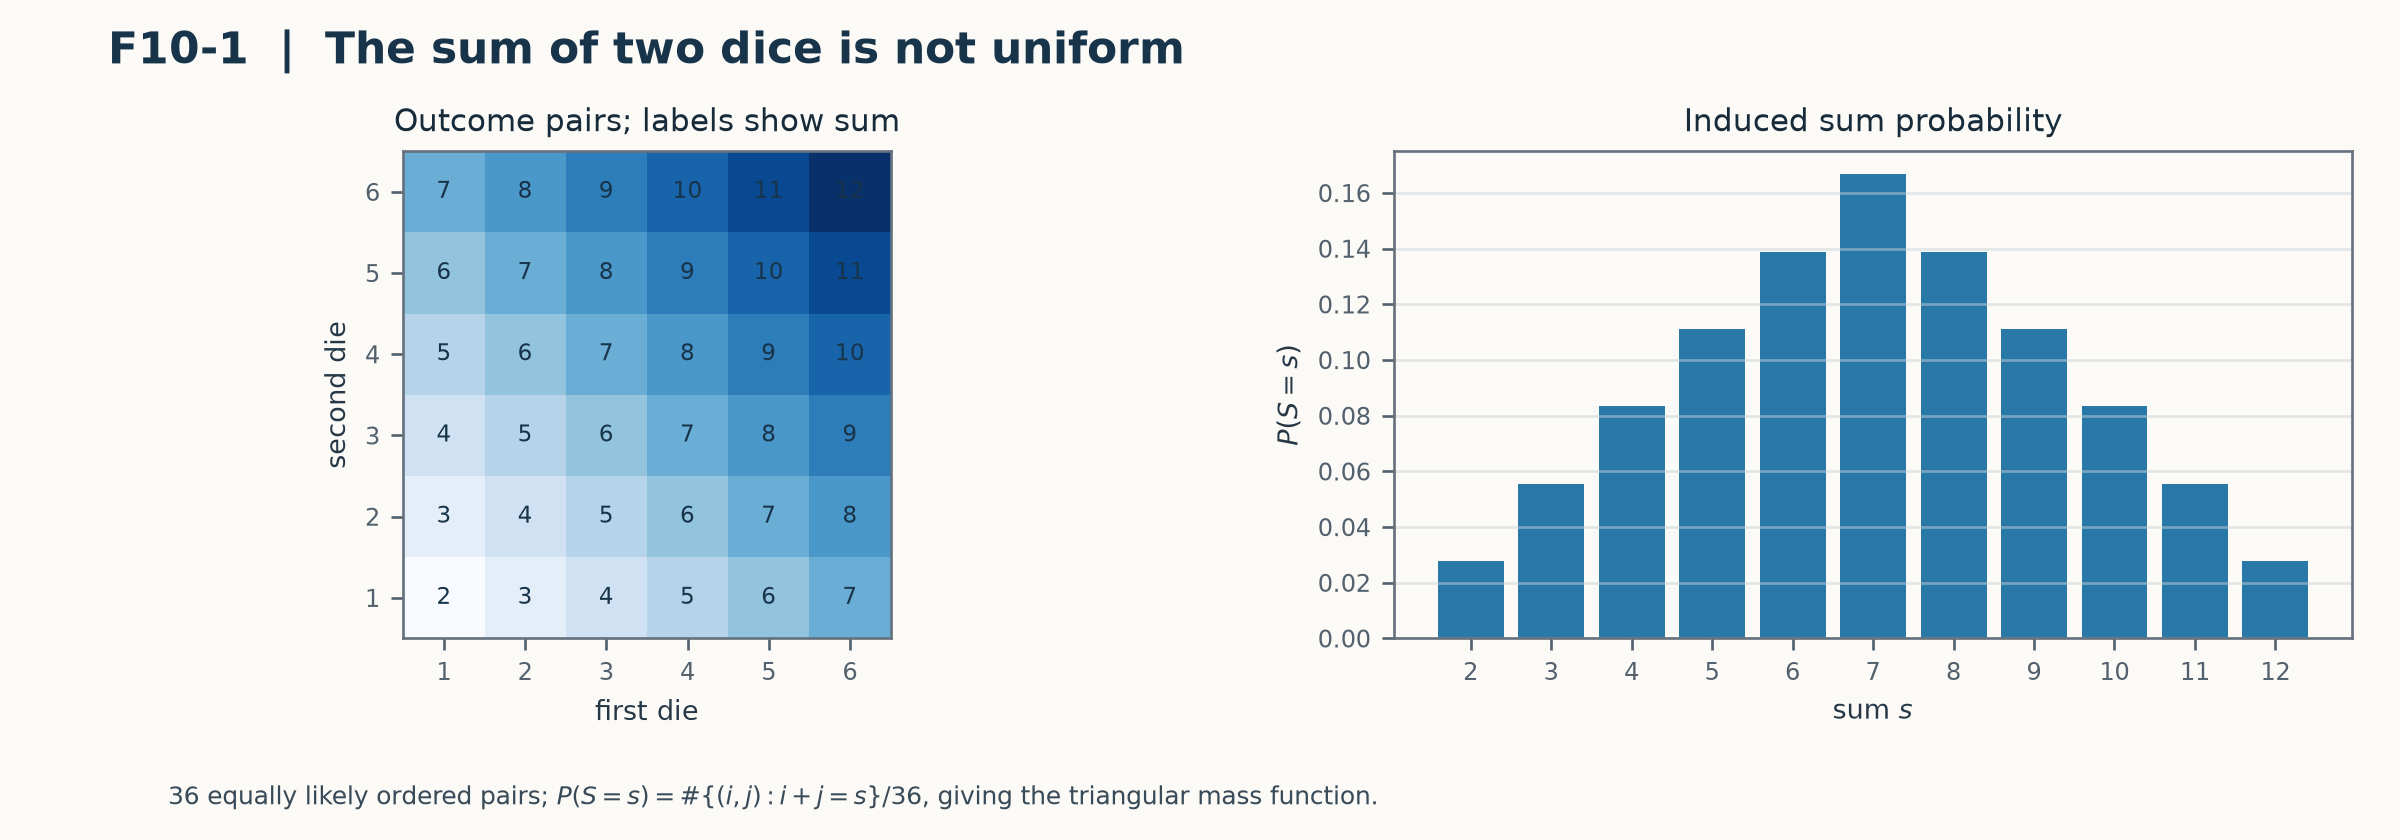
\includegraphics[keepaspectratio,alt={Visual Recall/Math Foundations/F10-1\_dice-sum.png}]{Visual Recall/Math Foundations/F10-1_dice-sum.png}}
\caption{Visual Recall/Math Foundations/F10-1\_dice-sum.png}
\end{figure}

\textbf{F10-1. Ordered outcomes and the exact two-dice sum PMF.} The supplied lesson already derives this example; the figure is a visual check of the 36 ordered pairs. PMF numerators sum to 36 and P(S=7)=1/6.

\begin{figure}
\centering
\pandocbounded{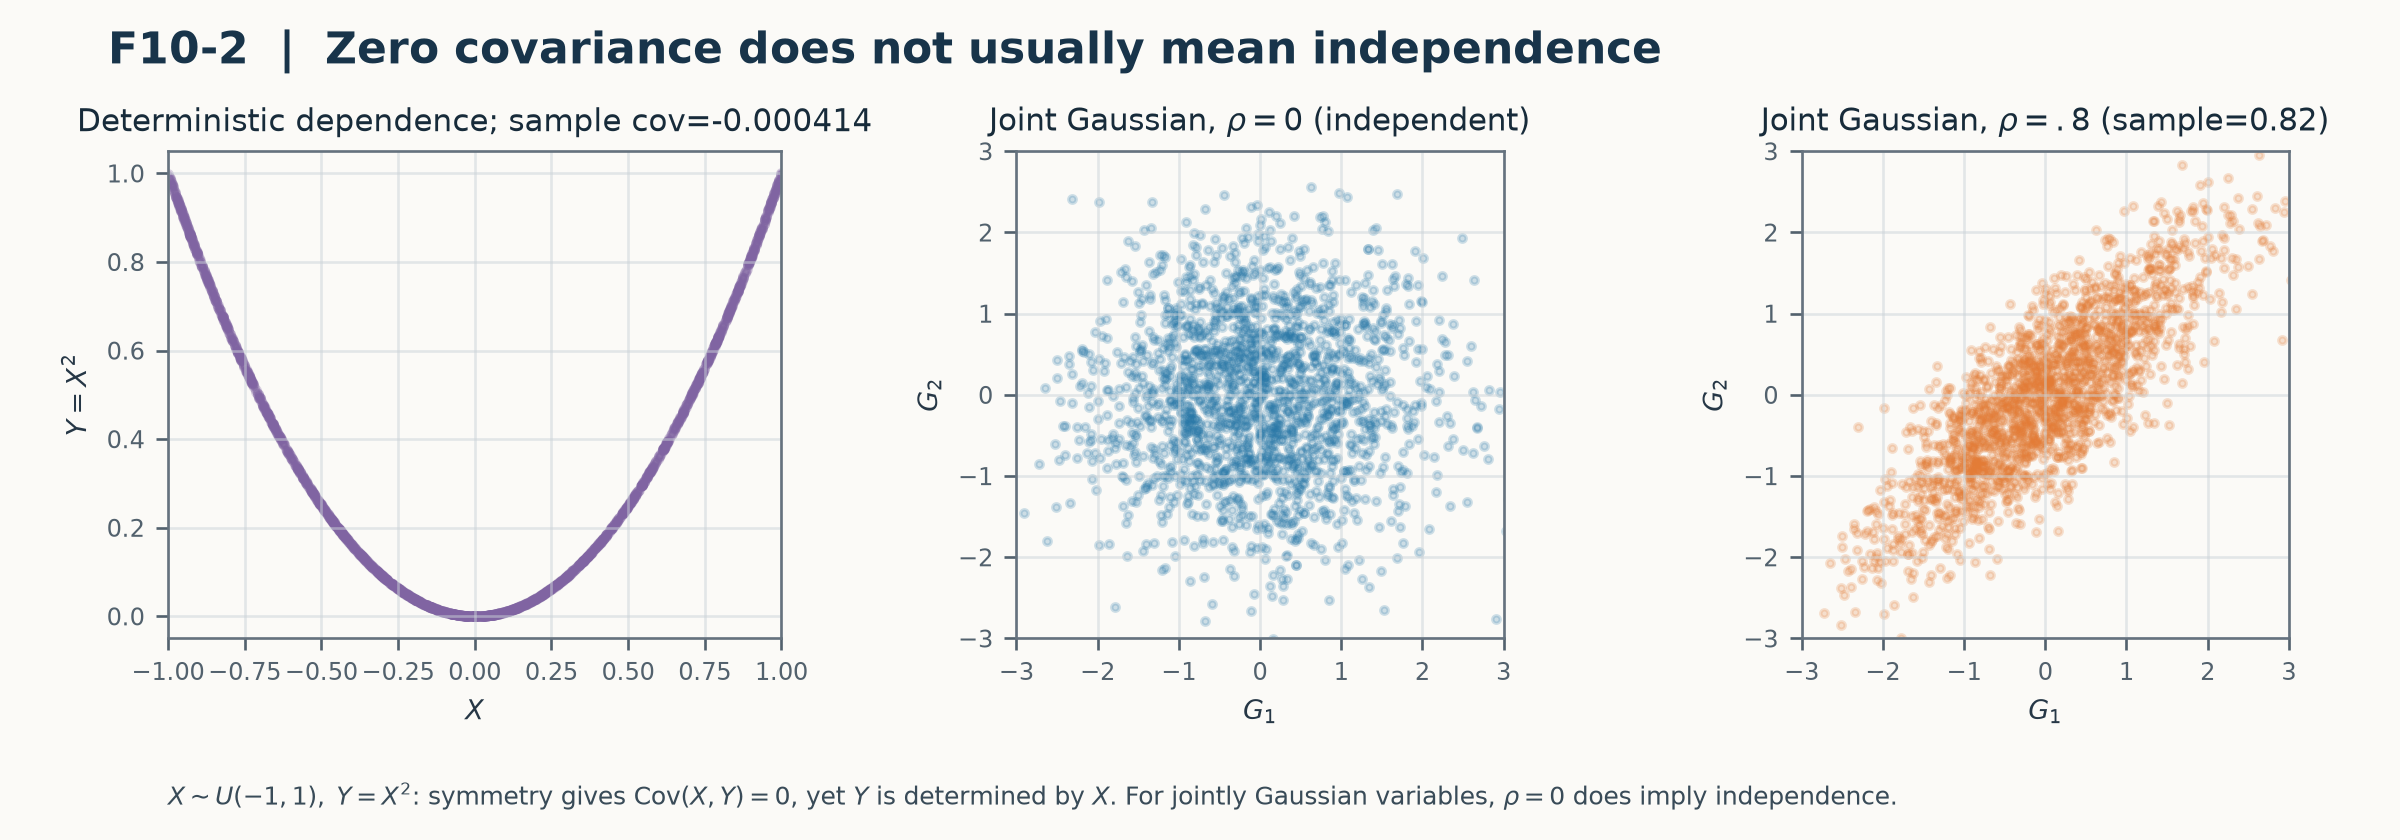
\includegraphics[keepaspectratio,alt={Visual Recall/Math Foundations/F10-2\_covariance-dependence.png}]{Visual Recall/Math Foundations/F10-2_covariance-dependence.png}}
\caption{Visual Recall/Math Foundations/F10-2\_covariance-dependence.png}
\end{figure}

\textbf{F10-2. Zero covariance need not mean independence.} For standard normal X, Cov(X,X squared)=0 by symmetry although X and X squared are dependent. Sample covariance is a finite-run witness.

\begin{figure}
\centering
\pandocbounded{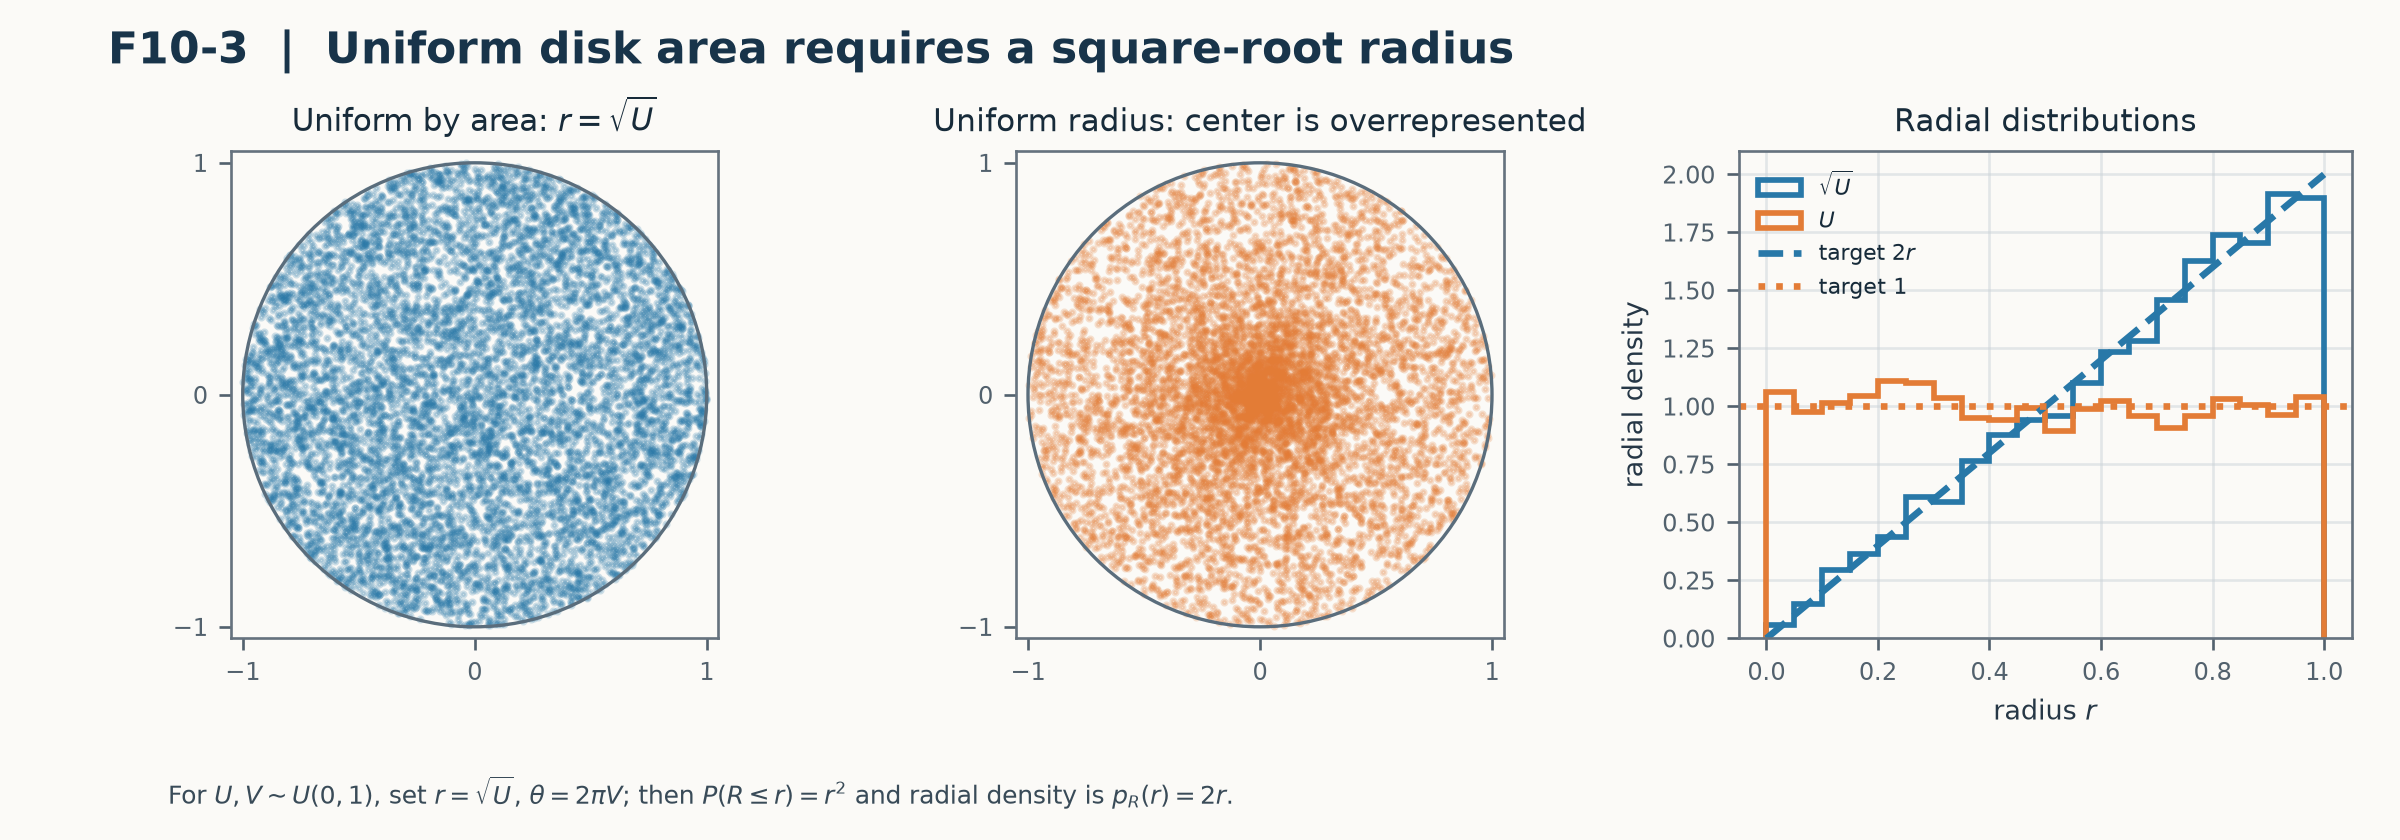
\includegraphics[keepaspectratio,alt={Visual Recall/Math Foundations/F10-3\_uniform-disk-sampling.png}]{Visual Recall/Math Foundations/F10-3_uniform-disk-sampling.png}}
\caption{Visual Recall/Math Foundations/F10-3\_uniform-disk-sampling.png}
\end{figure}

\textbf{F10-3. Uniform area sampling requires a square-root radial transform.} The theoretical mean radius is 2/3 for uniform area in the unit disk and 1/2 for uniform radius; plotted sample means are finite-run illustrations.

\begin{figure}
\centering
\pandocbounded{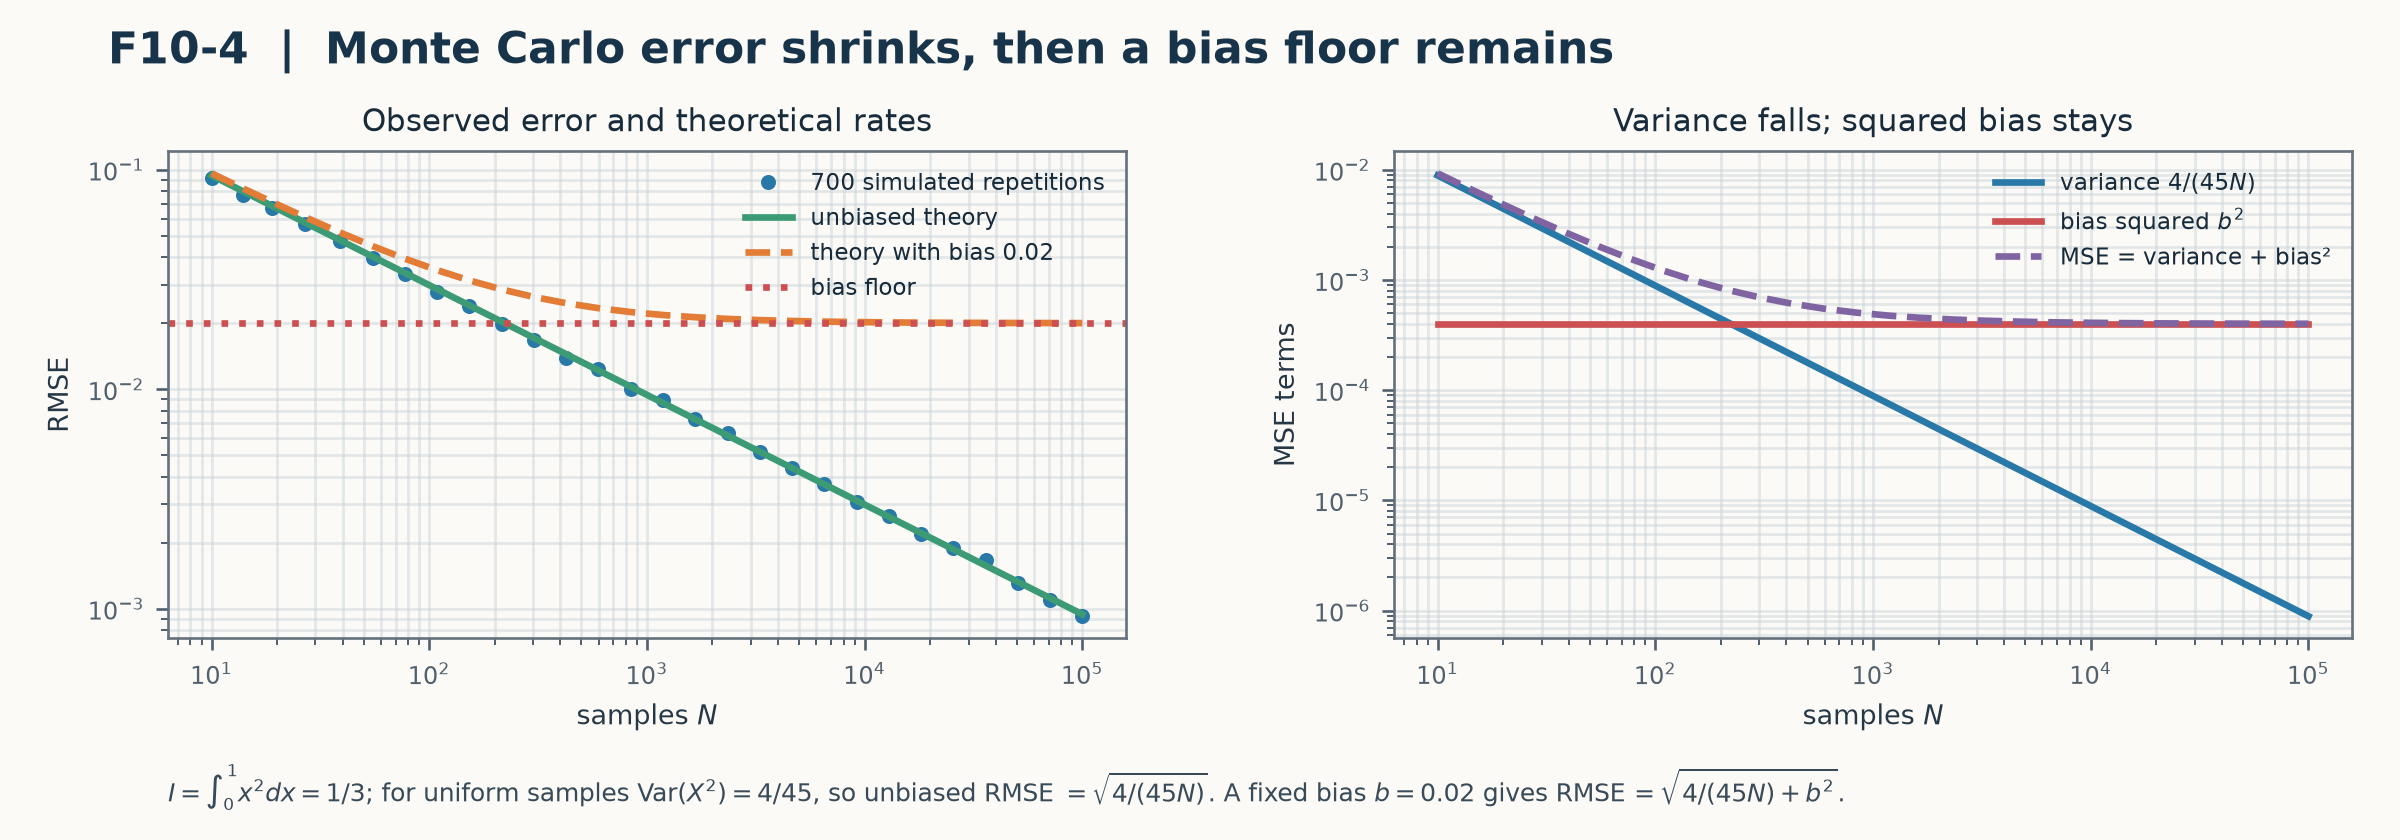
\includegraphics[keepaspectratio,alt={Visual Recall/Math Foundations/F10-4\_mc-error-bias-floor.png}]{Visual Recall/Math Foundations/F10-4_mc-error-bias-floor.png}}
\caption{Visual Recall/Math Foundations/F10-4\_mc-error-bias-floor.png}
\end{figure}

\textbf{F10-4. Monte Carlo random error and a fixed bias floor.} For the stated integral, unbiased RMSE falls with sample count while the biased estimator retains its offset.

\begin{figure}
\centering
\pandocbounded{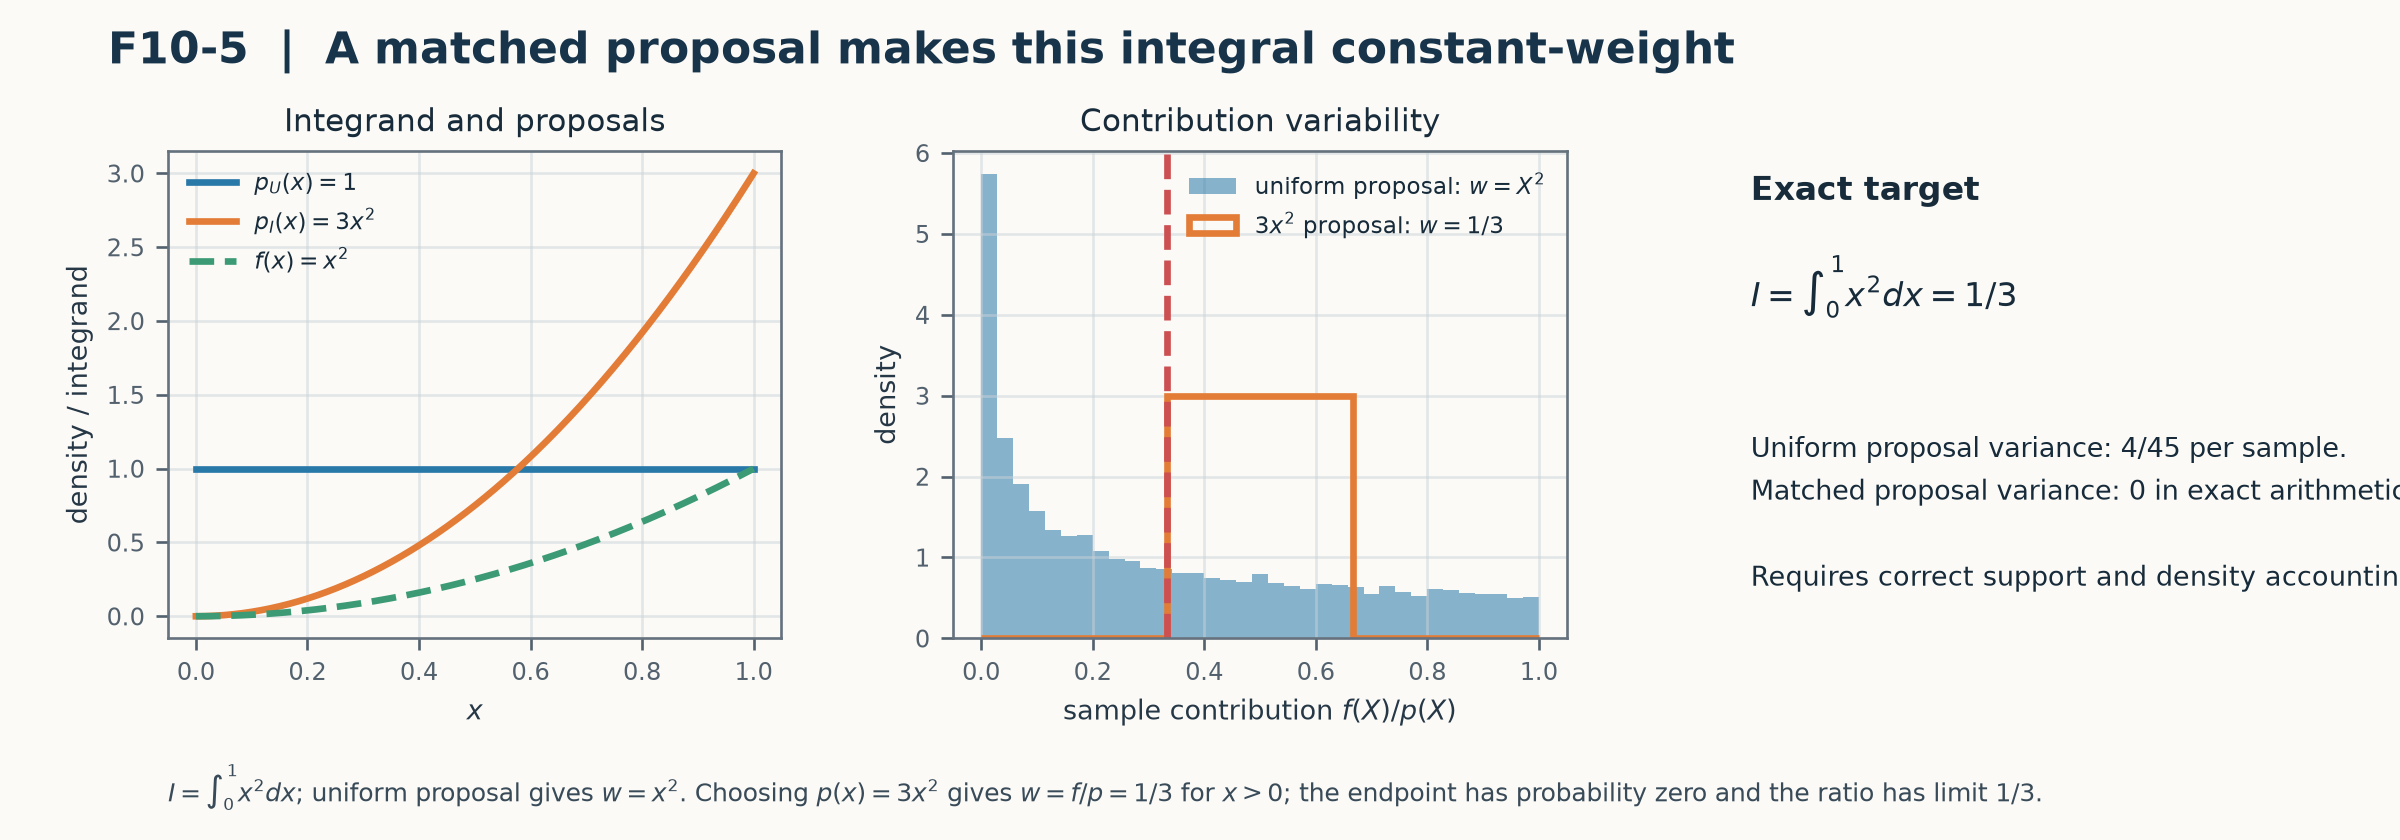
\includegraphics[keepaspectratio,alt={Visual Recall/Math Foundations/F10-5\_importance-constant-weight.png}]{Visual Recall/Math Foundations/F10-5_importance-constant-weight.png}}
\caption{Visual Recall/Math Foundations/F10-5\_importance-constant-weight.png}
\end{figure}

\textbf{F10-5. A matched importance proposal can make contributions constant.} For the stated nonnegative integrand and support, the matched proposal gives constant contributions; uniform-proposal variance is 4/45. This does not generalize to arbitrary signed integrands.

\begin{figure}
\centering
\pandocbounded{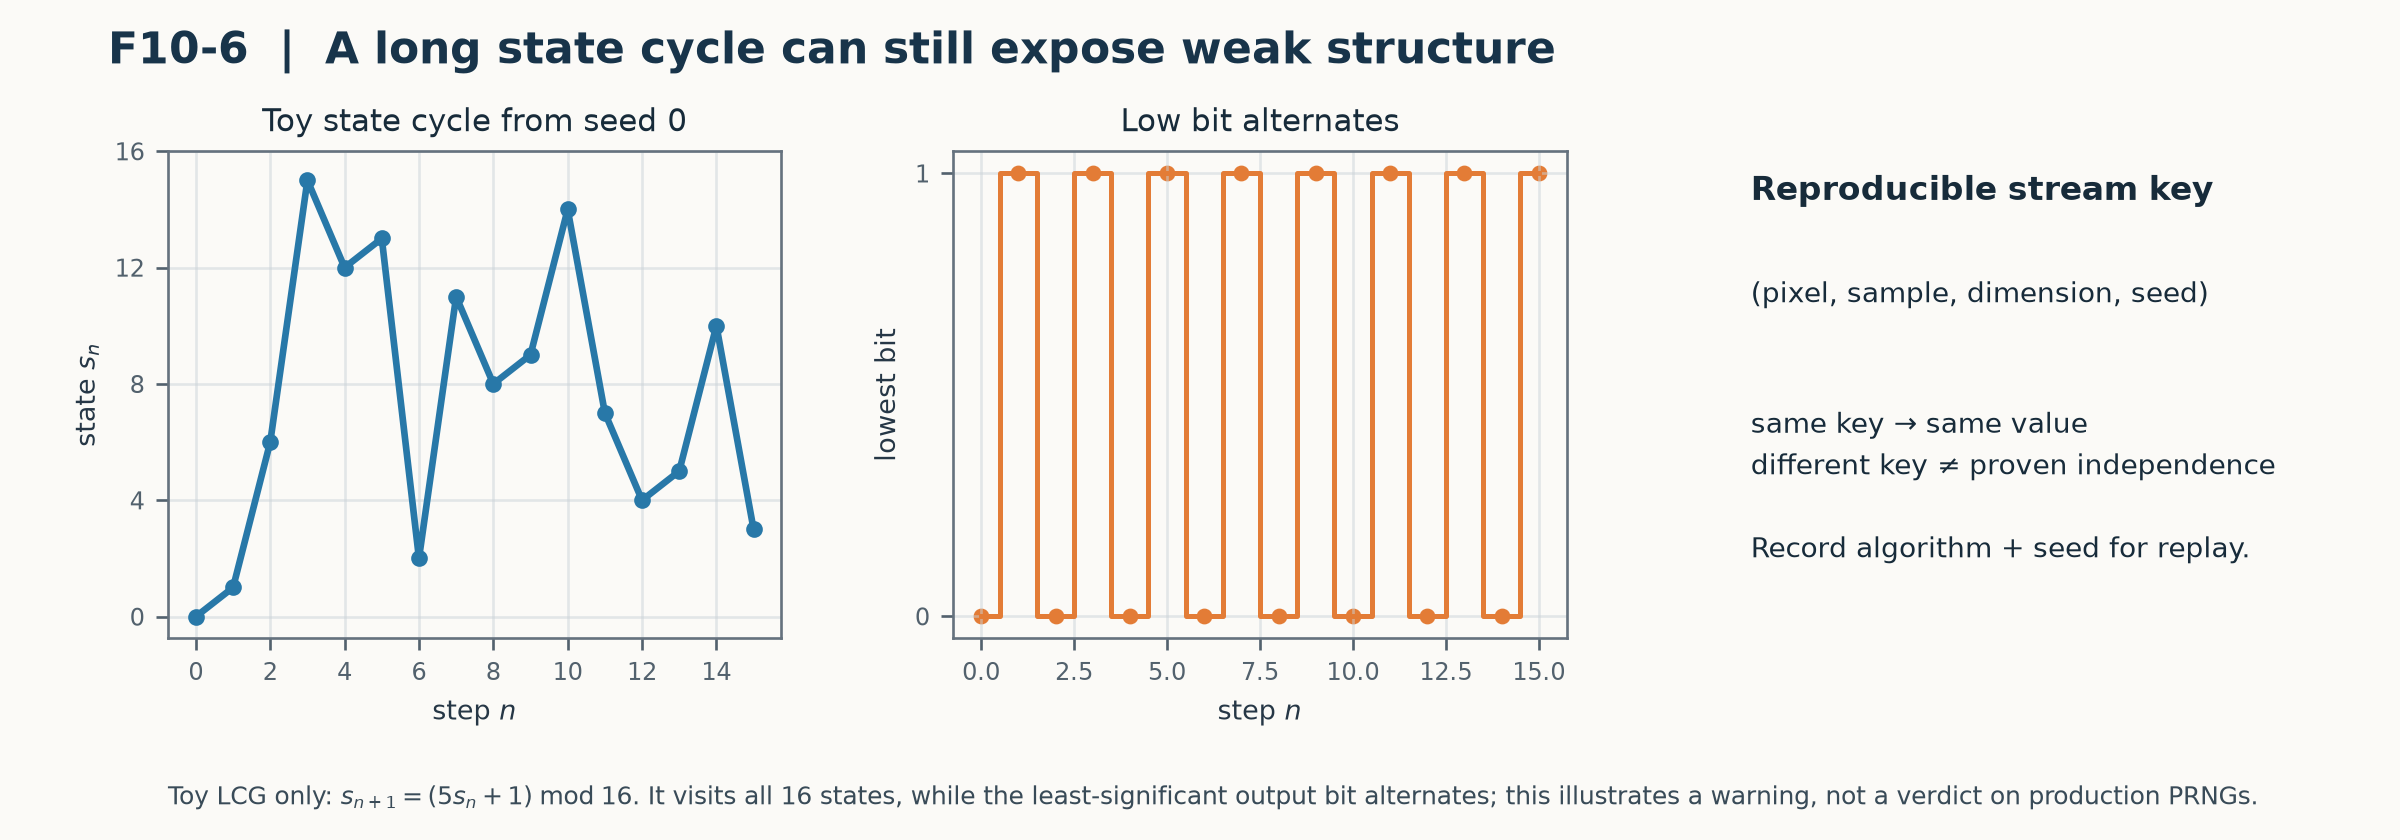
\includegraphics[keepaspectratio,alt={Visual Recall/Math Foundations/F10-6\_toy-lcg-stream.png}]{Visual Recall/Math Foundations/F10-6_toy-lcg-stream.png}}
\caption{Visual Recall/Math Foundations/F10-6\_toy-lcg-stream.png}
\end{figure}

\textbf{F10-6. A full-period toy LCG can still have a simple low-bit pattern.} For m=16, a=5, c=1, all 16 states are visited but the least-significant bit alternates. Full period does not imply good multidimensional quality. The keyed-input sketch indicates deterministic indexing only: a different key does not establish statistical independence or collision freedom.

\subsection{Phase 10 concept key map}\label{appendix-cb5af353ef77-phase-10-concept-key-map}

Use each keyword for the concept note and the adjacent section link for the full derivation or example.

{\def\LTcaptype{none} % do not increment counter
\begin{longtable}[]{@{}
  >{\raggedright\arraybackslash}p{(\linewidth - 2\tabcolsep) * \real{0.5000}}
  >{\raggedright\arraybackslash}p{(\linewidth - 2\tabcolsep) * \real{0.5000}}@{}}
\toprule\noalign{}
\begin{minipage}[b]{\linewidth}\raggedright
Concept keyword
\end{minipage} & \begin{minipage}[b]{\linewidth}\raggedright
Full teaching section
\end{minipage} \\
\midrule\noalign{}
\endhead
\bottomrule\noalign{}
\endlastfoot
{[}{[}Probability spaces, events, and conditioning & sample space{]}{]} \\
{[}{[}Random variables and probability laws & random law{]}{]} \\
{[}{[}Common probability distributions and their assumptions & normal distribution{]}{]} \\
{[}{[}Expectation, covariance, and dependence & first and second moments{]}{]} \\
{[}{[}Multivariate Gaussian distributions and whitening & normal vector{]}{]} \\
{[}{[}Conditional Gaussians and Schur complements & Schur complement covariance{]}{]} \\
{[}{[}Stateful pseudorandom generators and stream state & engine state{]}{]} \\
{[}{[}Stateless keyed sampling and reproducibility & counter-based RNG{]}{]} \\
{[}{[}Sampling quality: stratification, quasi-Monte Carlo, and blue noise & quasi-Monte Carlo{]}{]} \\
{[}{[}Inverse, rejection, and importance sampling & inverse transform{]}{]} \\
{[}{[}Online moments and Welford accumulation & online variance{]}{]} \\
{[}{[}Confidence intervals and sequential evidence & coverage interval{]}{]} \\
{[}{[}Robust summaries and error metrics & quantile{]}{]} \\
\end{longtable}
}

\subsection{The chain}\label{appendix-cb5af353ef77-the-chain}

Input uncertainty is amplified by conditioning; finite-precision algorithms add their own error. Keep \textbf{problem sensitivity}, \textbf{algorithm stability}, \textbf{approximation error}, and \textbf{sampling uncertainty} distinct. A small residual or update is evidence only when assumptions provide an error bound.

\subsection{Formula prompts}\label{appendix-cb5af353ef77-formula-prompts-1}

{\def\LTcaptype{none} % do not increment counter
\begin{longtable}[]{@{}
  >{\raggedright\arraybackslash}p{(\linewidth - 2\tabcolsep) * \real{0.5000}}
  >{\raggedright\arraybackslash}p{(\linewidth - 2\tabcolsep) * \real{0.5000}}@{}}
\toprule\noalign{}
\begin{minipage}[b]{\linewidth}\raggedright
Prompt
\end{minipage} & \begin{minipage}[b]{\linewidth}\raggedright
Rebuild
\end{minipage} \\
\midrule\noalign{}
\endhead
\bottomrule\noalign{}
\endlastfoot
First-order propagation & \(\Delta y\approx J_f(x)\Delta x\); define units and perturbation scale. \\
Multiplication & Relative errors approximately add to first order. \\
Summation & \(\gamma_n=nu/(1-nu)\); cancellation magnifies relative error. Pairwise depth is \(O(\log n)\); compensation tracks lost low-order bits. \\
Stable norm & \(m\sqrt{\sum_i(x_i/m)^2}\) with \(m=\max_i|x_i|\); handle \(m=0\). \\
Stable quadratic roots & Choose a noncancelling \(q\), then roots \(q/a\) and \(c/q\); separately handle degenerate and range cases. \\
Linear interpolation & \((1-t)y_0+ty_1\) for \(t\in[0,1]\); bounds require convex weights. \\
Bisection & Continuous sign-changing bracket; interval width halves each step. \\
Newton & \(x_{n+1}=x_n-f(x_n)/f'(x_n)\); local quadratic convergence needs a simple root and a good neighborhood. \\
Error balance & Truncation often falls with \(h^p\) while finite-difference roundoff grows like \(u/h\); balance before shrinking \(h\) indefinitely. \\
Convergence order & Compare \(Q_h,Q_{h/2},Q_{h/4}\); Richardson cancels a leading \(Ch^p\) term only in the asymptotic regime. \\
Log-sum-exp & \(m+\log\sum_i e^{a_i-m}\), \(m=\max_i a_i\); validate nonfinite/empty cases. \\
Stratified estimate & Sample every stratum and use weights matching its measure; arbitrary non-square grids must still cover the full domain. \\
\end{longtable}
}

\subsection{Checks before trusting a result}\label{appendix-cb5af353ef77-checks-before-trusting-a-result}

\begin{itemize}
\tightlist
\item
  State arithmetic assumptions (normal/subnormal, overflow, rounding mode) and data scale.
\item
  Check both residual/backward error and conditioning before interpreting forward accuracy.
\item
  Verify interpolation range, boundary policy, and parameter units.
\item
  Separate discretization, truncation, roundoff, and sampling error.
\item
  Fix a reproducible reduction tree or record seed, sample design, and uncertainty.
\item
  Test exact identities, invariants, edge cases, convergence order, and randomized strata.
\end{itemize}

\subsection{Continue in the volume}\label{appendix-cb5af353ef77-continue-in-the-volume}

\begin{itemize}
\tightlist
\item
  \href{../02-Foundations-II/main.pdf\#nameddest=02-foundations-ii-ch028-floating-point-answers-error-conditioning-stability-and-stable-arithmetic}{Error and arithmetic (02-Foundations-II, 02-foundations-ii-ch028-floating-point-answers-error-conditioning-stability-and-stable-arithmetic)}
\item
  \href{../02-Foundations-II/main.pdf\#nameddest=02-foundations-ii-ch028-reconstructing-values-and-curves-between-samples}{Interpolation and curves (02-Foundations-II, 02-foundations-ii-ch028-reconstructing-values-and-curves-between-samples)}
\item
  \href{../02-Foundations-II/main.pdf\#nameddest=02-foundations-ii-ch028-finding-roots-with-guarantees-and-convergence-checks}{Root solving (02-Foundations-II, 02-foundations-ii-ch028-finding-roots-with-guarantees-and-convergence-checks)}
\item
  \href{../02-Foundations-II/main.pdf\#nameddest=02-foundations-ii-ch029-separate-discretization-truncation-and-roundoff-measure-convergence}{Error sources and convergence (02-Foundations-II, 02-foundations-ii-ch029-separate-discretization-truncation-and-roundoff-measure-convergence)}
\item
  \href{../02-Foundations-II/main.pdf\#nameddest=02-foundations-ii-ch031-keep-probability-weights-stable-before-sampling}{Stable weights (02-Foundations-II, 02-foundations-ii-ch031-keep-probability-weights-stable-before-sampling)}
\item
  \href{../02-Foundations-II/main.pdf\#nameddest=02-foundations-ii-ch031-design-samples-without-replacement-stratified-and-low-discrepancy}{Sampling design (02-Foundations-II, 02-foundations-ii-ch031-design-samples-without-replacement-stratified-and-low-discrepancy)}
\item
  \href{../02-Foundations-II/main.pdf\#nameddest=02-foundations-ii-ch031-test-numerical-methods-and-benchmark-reproducibly}{Numerical tests (02-Foundations-II, 02-foundations-ii-ch031-test-numerical-methods-and-benchmark-reproducibly)}
\end{itemize}

\subsection{Numerical reliability figures and their explanations}\label{appendix-cb5af353ef77-numerical-reliability-figures-and-their-explanations}

\begin{itemize}
\item
  \href{../02-Foundations-II/main.pdf\#nameddest=02-foundations-ii-ch028-figure-n10-7-summation-is-an-algorithm-not-just-a-plus-sign}{N10-7 · Summation is an algorithm, not just a plus sign (02-Foundations-II, 02-foundations-ii-ch028-figure-n10-7-summation-is-an-algorithm-not-just-a-plus-sign)} --- Exact real sum is 10000. The three-term counterexample shows why Kahan is not an exact-arithmetic guarantee. Strict IEEE-style evaluation is assumed; reassociation can invalidate compensation.
\item
  \href{../02-Foundations-II/main.pdf\#nameddest=02-foundations-ii-ch028-figure-n10-8-more-polynomial-degree-does-not-guarantee-a-better-picture}{N10-8 · More polynomial degree does not guarantee a better picture (02-Foundations-II, 02-foundations-ii-ch028-figure-n10-8-more-polynomial-degree-does-not-guarantee-a-better-picture)} --- Both interpolants match every node. Their behaviour between nodes differs. Chebyshev extrema reduce this example's endpoint oscillation; this comparison is not a universal interpolation error bound.
\item
  \href{../02-Foundations-II/main.pdf\#nameddest=02-foundations-ii-ch028-figure-n10-9-bézier-and-hermite-can-tell-the-same-curve-story}{N10-9 · Bézier and Hermite can tell the same curve story (02-Foundations-II, 02-foundations-ii-ch028-figure-n10-9-bézier-and-hermite-can-tell-the-same-curve-story)} --- Use Hermite tangents 3(P1−P0) and 3(P3−P2) for this cubic Bézier curve. The control polygon bounds the curve through nonnegative weights summing to one; inner control points need not lie on the curve.
\item
  \href{../02-Foundations-II/main.pdf\#nameddest=02-foundations-ii-ch028-figure-n10-10-a-root-solver-needs-both-progress-and-a-safety-argument}{N10-10 · A root solver needs both progress and a safety argument (02-Foundations-II, 02-foundations-ii-ch028-figure-n10-10-a-root-solver-needs-both-progress-and-a-safety-argument)} --- The error comparison uses cos(x)−x with specified starting values. Bisection has a shrinking bracket; Newton and secant need additional hypotheses. The plotting floor is explicitly shown rather than interpreted as continuing convergence.
\item
  \href{../02-Foundations-II/main.pdf\#nameddest=02-foundations-ii-ch031-figure-n10-11-arbitrary-sample-counts-need-full-domain-support}{N10-11 · Arbitrary sample counts need full-domain support (02-Foundations-II, 02-foundations-ii-ch031-figure-n10-11-arbitrary-sample-counts-need-full-domain-support)} --- Left: choosing the first five of nine equal cells and averaging equally gives E{[}y{]} = 0.3, while the uniform-square value is 0.5. Right: one point per marginal bin is a midpoint illustration; randomized LHS jitters and permutes appropriately, and is not full multidimensional stratification.
\item
  \href{../02-Foundations-II/main.pdf\#nameddest=02-foundations-ii-ch028-figure-n10-12-algebraically-equal-formulas-can-have-unequal-numerical-error}{N10-12 · Algebraically equal formulas can have unequal numerical error (02-Foundations-II, 02-foundations-ii-ch028-figure-n10-12-algebraically-equal-formulas-can-have-unequal-numerical-error)} --- The reference uses 90-digit Decimal arithmetic and compares binary64 formulas for b from 100 to 10¹⁶. This bounded example illustrates cancellation, not a complete robust quadratic solver.
\end{itemize}

\subsection{Linked numerical concepts}\label{appendix-cb5af353ef77-linked-numerical-concepts}

\href{../02-Foundations-II/main.pdf\#nameddest=appendix-aa2bf0d79639}{Algorithmic stability (02-Foundations-II, appendix-aa2bf0d79639)} · \href{../02-Foundations-II/main.pdf\#nameddest=appendix-b9afba7f63e5}{Stable quadratic root evaluation (02-Foundations-II, appendix-b9afba7f63e5)} · \href{../02-Foundations-II/main.pdf\#nameddest=appendix-0c2a5f69851e}{Interpolation versus approximation (02-Foundations-II, appendix-0c2a5f69851e)} · \href{../02-Foundations-II/main.pdf\#nameddest=appendix-0a09b6dfdc86}{Tensor-product interpolation (02-Foundations-II, appendix-0a09b6dfdc86)} · \href{../02-Foundations-II/main.pdf\#nameddest=appendix-db3aef8f2fd6}{Cubic Hermite interpolation (02-Foundations-II, appendix-db3aef8f2fd6)} · \href{../02-Foundations-II/main.pdf\#nameddest=appendix-ddbec701898c}{Bézier curves and De Casteljau evaluation (02-Foundations-II, appendix-ddbec701898c)} · \href{../02-Foundations-II/main.pdf\#nameddest=appendix-f63eb850796d}{Bracketed and open root solvers (02-Foundations-II, appendix-f63eb850796d)} · \href{../02-Foundations-II/main.pdf\#nameddest=appendix-d83b0ad1be7f}{A posteriori error bounds for contractive iteration (02-Foundations-II, appendix-d83b0ad1be7f)} · \href{../02-Foundations-II/main.pdf\#nameddest=appendix-6b0648b2b8e8}{Discretization, truncation, and roundoff (02-Foundations-II, appendix-6b0648b2b8e8)} · \href{../02-Foundations-II/main.pdf\#nameddest=appendix-aca80b6bf17a}{Convergence order and Richardson extrapolation (02-Foundations-II, appendix-aca80b6bf17a)} · \href{../02-Foundations-II/main.pdf\#nameddest=appendix-d580b422240f}{Stable probability normalization and log-sum-exp (02-Foundations-II, appendix-d580b422240f)} · \href{../02-Foundations-II/main.pdf\#nameddest=appendix-184fcc411663}{Uniform shuffling without replacement (02-Foundations-II, appendix-184fcc411663)} · \href{../02-Foundations-II/main.pdf\#nameddest=appendix-1c5e85693a06}{Latin-hypercube sampling (02-Foundations-II, appendix-1c5e85693a06)} · \hyperref[appendix-31b8c295e05f]{Numerical error budgets} · \href{../02-Foundations-II/main.pdf\#nameddest=appendix-b9db93e28371}{Reproducible numerical benchmarking (02-Foundations-II, appendix-b9db93e28371)}

\subsection{Paired evidence --- retrieve the statistical unit}\label{appendix-cb5af353ef77-paired-evidence-retrieve-the-statistical-unit}

{\def\LTcaptype{none} % do not increment counter
\begin{longtable}[]{@{}
  >{\raggedright\arraybackslash}p{(\linewidth - 4\tabcolsep) * \real{0.3333}}
  >{\raggedright\arraybackslash}p{(\linewidth - 4\tabcolsep) * \real{0.3333}}
  >{\raggedright\arraybackslash}p{(\linewidth - 4\tabcolsep) * \real{0.3333}}@{}}
\toprule\noalign{}
\begin{minipage}[b]{\linewidth}\raggedright
Prompt
\end{minipage} & \begin{minipage}[b]{\linewidth}\raggedright
Short answer
\end{minipage} & \begin{minipage}[b]{\linewidth}\raggedright
Full commented witness
\end{minipage} \\
\midrule\noalign{}
\endhead
\bottomrule\noalign{}
\endlastfoot
What must survive a bootstrap or comparison? & The scene/run pairing; finite observations; and a test statistic whose result does not change with measurement units. & {[}{[}Continuous Notes/Computing Foundations - From Bits to C++ and Systems APIs\#A research claim needs more than a p-value \\
\end{longtable}
}
